\documentclass[letterpaper]{article}
\usepackage[utf8]{inputenc}
\usepackage[spanish,es-lcroman]{babel}
\usepackage{fancyhdr}
\usepackage{lastpage}
\usepackage{extramarks}
\usepackage[usenames,dvipsnames]{xcolor}
\usepackage{graphicx}
\usepackage{listings}
\usepackage{xparse}
\usepackage{courier}
\usepackage{float}
\usepackage{amsmath}
\usepackage{hyperref}
\usepackage{booktabs}


% Margenes
\topmargin=-0.45in
\evensidemargin=0in
\oddsidemargin=0in
\textwidth=6.5in
\textheight=9.0in
\headsep=0.25in


% Header y footer
\pagestyle{fancy}
\lhead{}
\chead{\guiaRamo\: \guiaTitulo} % Centro
\rhead{2015.2}
\lfoot{UTFSM-CSJ}
\cfoot{}
\rfoot{Página\ \thepage\ de\ \protect\pageref{LastPage}} % Pagina
\renewcommand\headrulewidth{0.4pt}
\renewcommand\footrulewidth{0.4pt}

\makeatletter
\newcommand{\titulo}[2]{%
  \vspace{#2}\noindent{#1}\vspace{\baselineskip}%
  \@afterindentfalse\@afterheading}
\makeatother


%------------------------------------------------------------------------
%	Meta Información
%------------------------------------------------------------------------
\newcommand{\guiaTitulo}{Tarea 2-3} % titulo del informe
\newcommand{\guiaFecha}{\today} % Fecha
\newcommand{\guiaRamo}{Seminario de Modelos y Métodos Cuantitativos} % Ramo
\newcommand{\guiaIniciales}{AL,JPEG} % Ramo
\newcommand{\guiaProfesor}{Andrés Moreira} % Profesor

%------------------------------------------------------------------------
%	Título
%------------------------------------------------------------------------
\title{
    \textmd{\textbf{\guiaRamo\\ \guiaTitulo}}\\
    \vspace{0.1in}
    \large{\textsc{Universidad Técnica Federico Santa María - Campus San Joaquín}}\\
    \normalsize\vspace{0.1in}\small{\guiaFecha}\\
    \vspace{0.1in}\large{\textit{Profesor \guiaProfesor}}
}
\author{
    \textsc{Juan Pablo Escalona G.} \\
    \small{juan.escalonag@alumnos.usm.cl} \\
    {\small 201073515-k}
    \and
     \textsc{Alonso Lepe M.} \\
    \small{alonso.lepe@alumnos.usm.cl}\\
    {\small 201173593-5}
\vspace{.5in}
}
\date{}

\begin{document}

\maketitle

\section{Pregunta 4}

\subsection{Grafico de la red}
\begin{figure}[H]
  \centering
  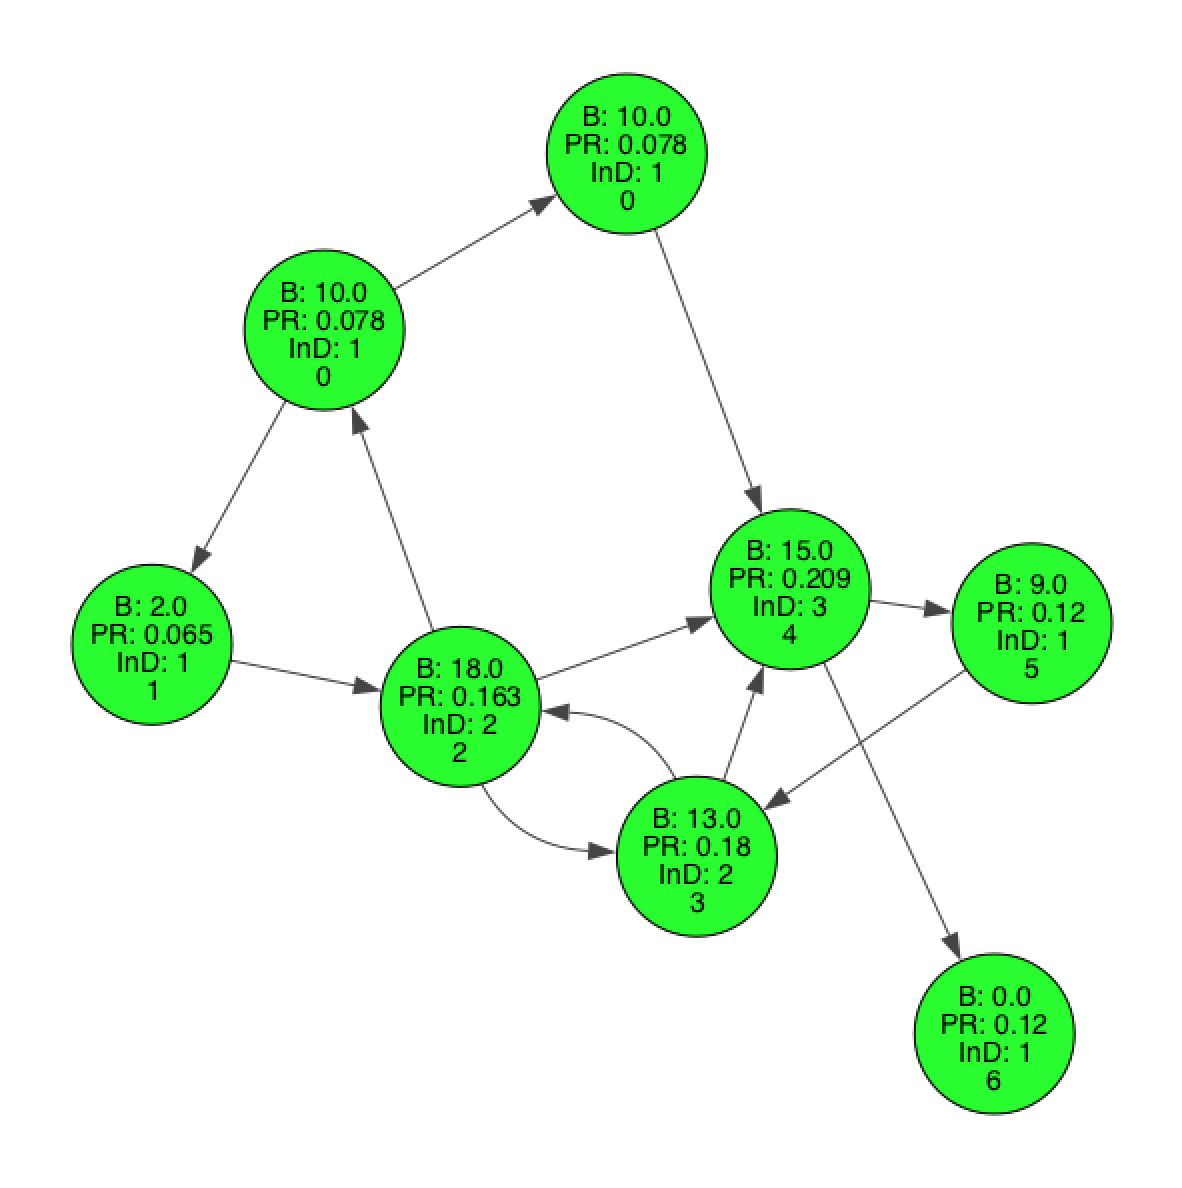
\includegraphics[width=.6\linewidth]{img/p4.png}
  \caption{Red chica dirigida. B: Betweenness, PR: PageRank, InD: Grado de entrada.}
\end{figure}


\begin{table}[H]
  \centering
  \renewcommand{\arraystretch}{1.1}
  \begin{tabular}{@{}ccccccccccc@{}}
    \toprule
       \multicolumn{3}{c}{\textsc{Grado Entrada}} & \phantom{abc} & \multicolumn{3}{c}{\textsc{Betweenness}} & \phantom{abc} & \multicolumn{3}{c}{\textsc{PageRank}}\\
       \cmidrule{1-3}\cmidrule{5-7}\cmidrule{9-11}
       Posición & Nodo & Valor & & Posición & Nodo & Valor & & Posición & Nodo & Valor\\
       \midrule
      1 & v5 & 3 &&  1 & v3 & 18 && 1 & v5 & 0.209 \\
      2 & v4 & 2 &&  2 & v5 & 15 && 2 & v4 & 0.180 \\
      2 & v3 & 2 &&  3 & v4 & 13 && 3 & v3 & 0.163 \\
      3 & v1 & 1 &&  4 & v1 & 10 && 4 & v6 & 0.120 \\
      3 & v2 & 1 &&  5 & v6 & 9  && 4 & v7 & 0.120 \\
      3 & v6 & 1 &&  6 & v8 & 3  && 5 & v1 & 0.078 \\
      3 & v7 & 1 &&  7 & v2 & 2  && 6 & v2 & 0.065 \\
      3 & v8 & 1 &&  8 & v7 & 0  && 6 & v8 & 0.065 \\
    \bottomrule
  \end{tabular}
  \caption{Ranking de cada índice para la red chica.}
\end{table}


\section{Referencias}
\section{Apéndice}

\end{document}
